% Hlavicka pro protokoly z fyzikalniho praktika.
% Verze pro: LaTeX
% Verze hlavicky: 22. 2. 2007
% Autor: Ustav fyziky kondenzovanych latek
% Ke stazeni: www.physics.muni.cz/ufkl/Vyuka/
% Licence: volne k pouziti, nejlepe k vcasnemu odevzdani protokolu z Vaseho mereni.

\documentclass[a4paper,11pt]{article}

% Kodovani (cestiny) v dokumentu: utf-8
%\usepackage[cp1250]{inputenc}	% Omezena stredoevropska kodova stranka, pouze MSW.
\usepackage[utf8]{inputenc}	% Doporucujeme pouzivat UTF-8 (unicode).

%%% Nemente:
\usepackage[margin=2cm]{geometry}
\newtoks\jmenopraktika \newtoks\jmeno \newtoks\datum
\newtoks\obor \newtoks\skupina \newtoks\rocnik \newtoks\semestr
\newtoks\cisloulohy \newtoks\jmenoulohy
\newtoks\tlak \newtoks\teplota \newtoks\vlhkost
\usepackage{amsmath}
\usepackage{mathtools}
\usepackage{graphicx}
\usepackage{multirow}
\graphicspath{ {./images/} }
%%% Nemente - konec.


%%%%%%%%%%% Doplnte pozadovane polozky:

\jmenopraktika={Fyzikální praktikum 2}  % nahradte jmenem vaseho predmetu
\jmeno={Artem Gorodilov}            % nahradte jmenem mericiho
\datum={20. ~listopadu  2023}        % nahradte datem mereni ulohy
\obor={Astrofyzika}                     % nahradte zkratkou vami studovaneho oboru
\skupina={Čt 8:00}            % nahradte dobou vyuky vasi seminarni skupiny
\rocnik={II}                  % nahradte rocnikem, ve kterem studujete
\semestr={I}                 % nahradte semestrem, ve kterem studujete

\cisloulohy={8}               % nahradte cislem merene ulohy
\jmenoulohy={Měření parametrů zobrazovacích soustav} % nahradte jmenem merene ulohy

\tlak={981}                   % nahradte tlakem pri mereni (v hPa)
\teplota={22.3}               % nahradte teplotou pri mereni (ve stupnich Celsia)
\vlhkost={43}               % nahradte vlhkosti vzduchu pri mereni (v %)

%%%%%%%%%%% Konec pozadovanych polozek.


%%%%%%%%%%% Uzitecne balicky:
\usepackage[czech]{babel}
\usepackage{graphicx}
\usepackage{amsmath}
\usepackage{xspace}
\usepackage{url}
\usepackage{indentfirst}
\usepackage{listings}
\usepackage{subcaption}
\usepackage{caption}
\usepackage{tabularx}
\usepackage[labelformat=parens,labelsep=quad,skip=3pt]{caption}

%%%%%% Zamezeni parchantu:
\widowpenalty 10000 \clubpenalty 10000 \displaywidowpenalty 10000
%%%%%% Parametry pro moznost vsazeni vetsiho poctu obrazku na stranku
\setcounter{topnumber}{3}	  % max. pocet floatu nahore (specifikace t)
\setcounter{bottomnumber}{3}	  % max. pocet floatu dole (specifikace b)
\setcounter{totalnumber}{6}	  % max. pocet floatu na strance celkem
\renewcommand\topfraction{0.9}	  % max podil stranky pro floaty nahore
\renewcommand\bottomfraction{0.9} % max podil stranky pro floaty dole
\renewcommand\textfraction{0.1}	  % min podil stranky, ktery musi obsahovat text
\intextsep=8mm \textfloatsep=8mm  %\intextsep pro ulozeni [h] floatu a \textfloatsep pro [b] or [t]

% Tecky za cisly sekci:
\renewcommand{\thesection}{\arabic{section}.}
\renewcommand{\thesubsection}{\thesection\arabic{subsection}.}
% Jednopismenna mezera mezi cislem a nazvem kapitoly:
\makeatletter \def\@seccntformat#1{\csname the#1\endcsname\hspace{1ex}} \makeatother

\begin{document}

\thispagestyle{empty}

{
\begin{center}
\sf 
{\Large Ústav fyzikální elektroniky PřF MU} \\
\bigskip
{\huge \bfseries FYZIKÁLNÍ PRAKTIKUM} \\
\bigskip
{\Large \the\jmenopraktika}
\end{center}

\bigskip

\sf
\noindent
\setlength{\arrayrulewidth}{1pt}
\begin{tabular*}{\textwidth}{@{\extracolsep{\fill}} l l}
\large {\bfseries Zpracoval:}  \the\jmeno & \large  {\bfseries Naměřeno:} \the\datum\\[2mm]
\large  {\bfseries Obor:} \the\obor  \hspace{40mm}  {\bfseries Skupina:} \the\skupina %
%{\bfseries Ročník:} \the\rocnik \hspace{5mm} {\bfseries Semestr:} \the\semestr  
&\large {\bfseries Testováno:}\\
\\
\hline
\end{tabular*}
}

\bigskip

{
\sf
\noindent \begin{tabular}{p{3cm} p{0.6\textwidth}}
\Large  Úloha č. {\bfseries \the\cisloulohy:} \par
\smallskip
$T=\the\teplota$~$^\circ$C \par
$p=\the\tlak$~hPa \par
$\varphi=\the\vlhkost$~\%
&\Large \bfseries \the\jmenoulohy  \\[2mm]
\end{tabular}
}

\vskip1cm
    \begin{minipage}[t]{0.5\textwidth} 
        \section{Zadání}
            Určit ohniskovou vzdálenost k tenké spojce. 
            \par Určit ohniskovou vzdálenost k tenké spojce.
            \par Určit index lomu z ohniskové vzdálenosti a zakřivení čočky.
        \section{Teorie}
            \subsection{Ohnisková vzdálenost tenké spojky a rozptylky}
                Dopadá-li paprsek světla na optickou soustavu rovnoběžně s optickou osou, sbíhají se paprsky v ohnisku $F'$. Jestliže svazek paprsků vychází z předmětového ohniska $F$, přemění se po průchodu soustavou na rovnoběžný svazek světla. Schéma je vidět na obrázku (1). Předmětový a obrazový prostor lze charakterizovat souřadnicovými systémy, jejichž počátek je ve středu objektivu. Vpravo od počátku souřadného systému je (+) a vlevo je (-).
                \par Ohnisková vzdálenost $f'$ se vypočítá podle následujícího vzorce: 
                \begin{equation}
                    f' = \frac{aa'}{a-a'}
                \end{equation}
                kde $a$ je vzdálenost předmětu a $a'$ je vzdálenost obrazu.
                \par Když se zobrazí objekt o velikosti $y$, získá se obraz o velikosti $y'$, poměr těchto dvou veličin, což je zvětšeni, lze zjistit ze vzorce: 
                \begin{equation}
                    \beta = \frac{y'}{y} = \frac{a'}{a}
                \end{equation}
    \end{minipage}
    \hspace{10pt}
    \begin{minipage}[t]{0.5\textwidth} 
                \vspace{0pt}   
                \par \centering
                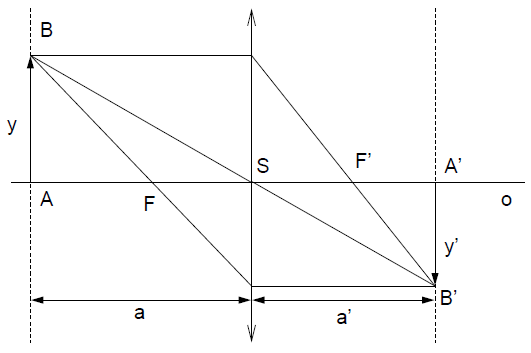
\includegraphics[scale=0.35]{prim}
                \captionsetup{justification=centering, font=footnotesize}
                \captionof{figure}{Přímé měření ohniskové vzdálenosti tenké čočky.}
                \label{fig:prim}
                \vspace{10pt}
                \raggedright
                \vspace{10pt}
                \par Potom lze ohniskovou vzdálenost $f_z'$ vypočítat podle vzorce:
                \begin{equation}
                    f_z' = \frac{a'}{1 - \beta}
                \end{equation}
                Kromě toho lze ohniskovou vzdálenost $f_B'$ určit Besselovou metodou, která je definována vztahem:
                \begin{equation}
                    f_B' = \frac{d^2 - \Delta^2}{4d}
                \end{equation}
                kde: 
                \begin{equation}
                    d = \vert a_1 \vert + \vert a_1' \vert = \vert a_2 \vert + \vert a_2' \vert
                \end{equation}
                \begin{equation}
                    d^2-\Delta^2 = 4a_1 a_1' = 4a_2 a_2'
                \end{equation}   
                Schéma je vidět na obrázku (2).
                \vspace{0pt}   
                \par \centering
                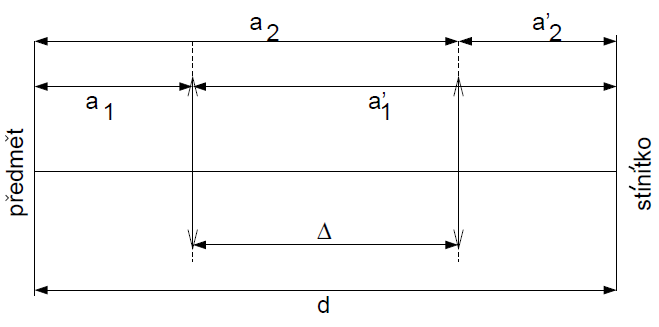
\includegraphics[scale=0.35]{bessel}
                \captionsetup{justification=centering, font=footnotesize}
                \captionof{figure}{Besselova metoda měření ohniskové vzdálenosti.}
                \label{fig:bessel}
                \vspace{10pt}
                \raggedright
                \vspace{10pt}      
    \end{minipage}
\newpage
    \begin{minipage}[t]{0.5\textwidth} 
                Obrazovka musí mít pevnou vzdálenost. V tomto případě budou existovat pouze 2 polohy čočky, při kterých bude obraz na stínítku ostrý.
                \par Při použití rozptylky se vždy získá imaginární obraz skutečného objektu. Pak se vzdálenost k předmětu $a$ a jeho obrazu $a'$ rovnají, resp:
                \begin{equation}
                    a = A - R
                \end{equation}
                \begin{equation}
                    a' = A' - R
                \end{equation}
                kde $A$ a $A'$ jsou poloha obrazu spojky a obrazu rozptylky resp., a $R$ je poloha rozptylky.
                Schéma je vidět na obrázku (3).
                \vspace{10pt}   
                \par \centering
                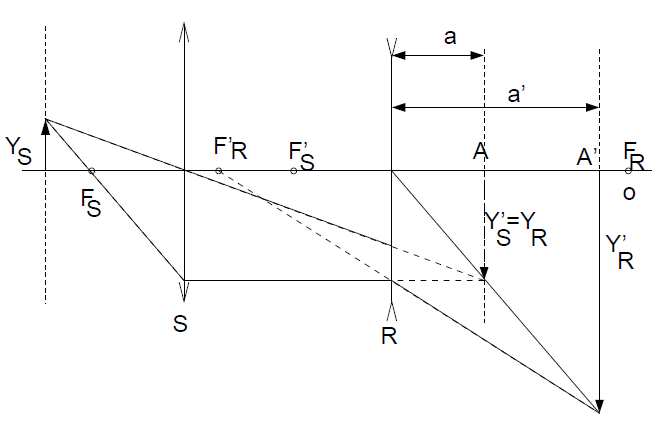
\includegraphics[scale=0.4]{rozp}
                \captionsetup{justification=centering, font=footnotesize}
                \captionof{figure}{Měření ohniskové vzdálenosti rozptylky.}
                \label{fig:rozp}
                \vspace{10pt}
                \raggedright
            \subsection{Index lomu}
                Pomocí sférometru změříme index lomu, který měří výchylku čočky. U rozptylky bude výchylka kladná a u rozptylky záporná. Index lomu $n$ se vypočítá podle vzorce (9): 
                \begin{equation}
                    n = 1 + \frac{1}{f \left( \frac{1}{r_1} - \frac{1}{r_2} \right)}
                \end{equation}
                kde $f$ je ohnisková vzdálenost čočky a $r_1$ a $r_2$ je poloměry křivosti čoček.
                \par Poloměr křivosti čočky se vypočítá podle vzorce:
                \begin{equation}
                    r = \frac{z^2+h^2}{2h}
                \end{equation}
                kde $z$ je poloměr báze sférometru a $h$ je vzdálenost mezi stínítkem a čočkou.
            \end{minipage}
    \hspace{10pt}
    \begin{minipage}[t]{0.5\textwidth} 
        \section{Měření}  
            \subsection{Ohnisková vzdálenost tenké spojky a rozptylky}
                Změřme vzdálenost objektu $a$ a vzdálenost obrázku $a'$ pro pět různých poloh stínítka $l$ a čočky. Poté použijeme vzorce (1), (2), (3) a (4) k určení ohniskové vzdálenosti $f$, $f_z$ a $f_B$ a zvětšeni $\beta$ pomocí tří různých metod. Výsledky jsou uvedeny v tabulce (1).
                Odtud zjistíme hodnoty $f'$, $f_z'$ a $f_B'$ a jejich chyby: 
                \begin{center}
                    $f'$ = 16.0(6) [cm]
                    \vspace{5pt}
                    \par $f_z'$ = 16.0(6) [cm]
                    \vspace{5pt}
                    \par $f_B'$ = 16.38(3) [cm]
                \end{center}
                S toho zjistíme hodnotu ohniskové vzdálenosti $f$ a její chybu:
                \begin{center}
                    $f_{conv, mean}'$ = 16.1(1) [cm]
                \end{center}
                Dále jsme změřili ohniskovou vzdálenost konkávní čočky. Za tímto účelem jsme změřili vzdálenost od objektu k obrazu získanému konvexní čočkou $A$ a vzdálenost od objektu k obrazu získanému konkávní čočkou $A'$. Měření byla provedena pro čtyři kobminace poloh konkávní čočky, konvexní čočky a obrazovky. Poté jsme vypočítali hodnoty $a$ a $a'$ podle vzorců (7) a (8) a vypočítali ohniskovou vzdálenost podle vzorce (1). Výsledky jsou shrnuty v tabulce (2).     
                \begin{center}
                    $f_{conc, mean}'$ = -(30 $\pm$ 10) [cm]
                \end{center}
                \subsection{Index lomu}
                Dále určíme index lomu $n$ pro konvexní a konkávní čočky. 
                \par Nejprve změříme vnější a vnitřní průměr báze sférometru $z_{out}$ a $z_{in}$ a poté jej použijeme k měření průhybu čočky $h$.
                \par Výsledky měření pro konvexní čočku a pro konkávní čočku jsou v tabulce (4).    
    \end{minipage}   
            \begin{table}[b]
                \centering
                \begin{tabular}{|c|c|c|c|c|c|c|}
                    \hline
                    $l$ [cm] & $a$ [cm] & $a'$ [cm] & $\beta$ & $f'$ [cm] & $f_z'$ [cm] & $f_b'$ [cm] \\
                    \hline
                    66.0(1) & 28.5(2) & 37.5(2) & -1.31(2) & 16.18(4) & 16.18(4) & 16.32(3)\\
                    \hline
                    72.0(1) & 24.4(2) & 47.6(2) & -1.95(2) & 16.12(6) & 16.12(6) & 16.40(5)\\
                    \hline
                    76.0(1) & 22.7(1) & 53.3(2) & -2.35(2) & 15.91(6) & 15.91(6) & 16.34(5)\\
                    \hline
                    82.0(1) & 21.7(1) & 60.3(2) & -2.78(2) & 15.94(7) & 15.94(7) & 16.38(5)\\
                    \hline
                    88.1(1) & 20.1(2) & 67.2(2) & -3.22(3) & 15.92(8) & 15.92(8) & 16.46(7)\\
                    \hline
                \end{tabular}
                \captionsetup{justification=centering, font=footnotesize}
                \captionof{table}{Vzdálenosti objektu $a$ a obrázku $a'$, ohniskové vzdálenosti $f$, $f_z$ a $f_B$ a zvětšeni $\beta$}
                \raggedright
            \end{table}
\newpage
            \begin{table}[t]   
                \centering
                \begin{tabular}{|c|c|c|c|c|c|c|}
                    \hline
                    $A$ [cm] & $A'$ [cm] & $S$ [cm] & $R$ [cm] & $a'$ [cm] & $a$ [cm] & $f$ [cm] \\
                    \hline
                    62.0(1) & 71.0(1) & 28.0(1) & 49.19(1) & 21.8(2) & 12.8(2) & -30.9(8)\\
                    \hline
                    72.0(1) & 81.0(1) & 24.0(1) & 59.09(2) & 21.9(2) & 12.9(2) & -31.2(9)\\
                    \hline
                    78.0(1) & 89.0(1) & 22.0(1) & 63.90(7) & 25.0(7) & 14.0(7) & -32.0(2.5)\\
                    \hline
                    82.0(1) & 91.0(1) & 20.0(1) & 70.08(2) & 20.9(2) & 11.9(2) & -27.5(9)\\
                    \hline
                \end{tabular}
                \captionsetup{justification=centering, font=footnotesize}
                \captionof{table}{Vzdálenosti objektu $A$ a obrázku $A'$, vzdálenost předmětu od zakřivené čočky $S$, vzdálenost předmětu od konkávní čočky $R$.}
                \vspace{10pt}
                \begin{tabular}{|c|c|c|c|c|c|}
                    \hline
                    $z_{in}$ [mm] & $z_{out}$ [mm] & $h_{conc, 1}$ [mm] & $h_{conc, 2}$ [mm] & $h_{conv, 1}$ [mm] & $h_{conv, 2}$ [mm] \\
                    \hline
                    17.283(1) & 18.602(1) & -0.502(1) & -0.505(1) & 1.838(1) & 0.005(1)\\
                    \hline
                    17.377(1) & 18.603(1) & -0.505(1) & -0.506(1) & 1.836(1) & 0.004(1)\\
                    \hline
                    17.382(1) & 18.602(1) & -0.504(1) & -0.504(1) & 1.838(1) & 0.005(1)\\
                    \hline
                    17.382(1) & 18.602(1) & -0.503(1) & -0.505(1) & 1.839(1) & 0.004(1)\\
                    \hline
                    17.381(1) & 18.601(1) & -0.503(1) & -0.509(1) & 1.838(1) & 0.004(1)\\
                    \hline
                    17.383(1) & 18.601(1) & -0.503(1) & -0.509(1) & 1.839(1) & 0.005(1)\\
                    \hline
                    17.361(1) & 18.602(1) & -0.504(1) & -0.507(1) & 1.837(1) & 0.005(1)\\
                    \hline
                    17.368(1) & 18.602(1) & -0.503(1) & -0.506(1) & 1.840(1) & 0.006(1)\\
                    \hline
                    17.388(1) & 18.602(1) & -0.503(1) & -0.511(1) & 1.832(1) & 0.005(1)\\
                    \hline
                    17.373(1) & 18.601(1) & -0.503(1) & -0.509(1) & 1.840(1) & 0.005(1)\\
                    \hline
                \end{tabular}
                \captionsetup{justification=centering, font=footnotesize}
                \captionof{table}{Vnější a vnitřní průměr báze sférometru $z_{out}$ a $z_{in}$ a průhyb čočky $h$}
                \vspace{10pt}
            \end{table}
    \begin{minipage}[t]{0.5\textwidth}
                \par Z měření zjistíme průměrné hodnotu poloměru báze sférometru $z$ a také hodnoty průhybu pro obě strany čočky $h_{conv, 1}$, $h_{conv, 2}$ a $h_{conc, 1}$, $h_{conc, 1}$. Potom podle vzorce (10) zjistíme poloměr křivosti pro obě čočky $r_{conv}$ a $r_{conc, 1}$, $r_{conc, 2}$:
                \begin{center}
                    $z$ = 17.98(5) [mm]
                    \vspace{15pt}
                    \par $h_{conv, 1}$ = 1.84(3) [mm]
                    \vspace{5pt}
                    \par $h_{conv, 2}$ = 0.01(3) [mm]
                    \vspace{5pt}
                    \par $r_{conv}$ = 89.2(2) [mm]
                    \vspace{15pt}
                    \par $h_{conc, 1}$ = 0.50(3) [mm]
                    \vspace{5pt}
                    \par $h_{conc, 2}$ = 0.51(3) [mm]
                    \vspace{5pt}
                    \par $r_{conc, 1}$ = (322 $\pm$ 20) [mm]
                    \vspace{5pt}
                    \par $r_{conc, 2}$ = (319 $\pm$ 20) [mm]
                    \vspace{5pt}
                    \par $r_{conc}$ = (322 $\pm$ 15) [mm]
                \end{center}
                Potom podle vzorce (9) zjistíme hodnotu indexu lomu $n_{conc}$ a $n_{conc}$ pro obě čočky: 
                \begin{center}
                    $n_{conv}$ = 1.5(1)
                    \vspace{5pt}
                    \par $n_{conc}$ = 2.1(4)
                \end{center}
                \vspace{10pt}
                K výpočtu veličin a jejich nejistot byla použita knihovna Uncertinties pro Python: \href{pypi.org/project/uncertainties}. Kód je přiložen k protokolu. Chyby byly rozšířeny o Studentův koeficient (2-Tail Confidence Level) s ohledem na stupně volnosti pro každou hodnotu, pro interval spolehlivosti 99\%. 
    \end{minipage}
    \hspace{10pt}  
    \begin{minipage}[t]{0.5\textwidth} 
                \section{Závěr}  
                    \subsection{Ohnisková vzdálenost tenké spojky a rozptylky}
                        Pomocí tří různých metod jsme zjistili hodnoty ohniskové vzdálenosti pro konvexní čočku podle vzorců (1), (2) a (3): $f'$ = 16.0(5) [cm], $f_z'$ = 16.0(5) [cm], $f_B'$ = 16.4(3) [cm]. Je vidět, že vypočtená hodnota ohniskové vzdálenosti pomocí Besselovy metody je přesnější.
                    \subsection{Index lomu}
                        Pomocí sférometru jsme změřili průměr báze $z$ a průhyb čočky $h$ pro konvexní a konkávní čočky. Potom jsme zjistili poloměr křivosti $r$ pro obě čočky. Z těchto hodnot jsme vypočítali index lomu $n_{conv}$ = 1.6(1) a $n_{conc}$ = 2.1(4) pro konvexní a konkávní čočky resp. 
                        \par Hodnoty indexu lomu se liší od tabulkových hodnot. To může být způsobeno tím, že čočky nejsou ideální a mají určitou chybu. 
    \end{minipage}
\newpage
    \par K výpočtu chyb byl použit následující kód: 
    \begin{lstlisting}[language=Python, basicstyle=\tiny, breaklines=true, postbreak=\mbox{\textbackslashspace}]
        #Importing the libraries

        import matplotlib.pyplot as plt
        import numpy as np
        import pandas as pd
        from scipy import stats
        from scipy.stats import t as t 
        from scipy.optimize import curve_fit
        from uncertainties import *
        from uncertainties.umath import *

        #Reading data

        im70 = pd.read_excel('data/Im70.xlsx')
        im76 = pd.read_excel('data/Im76.xlsx')
        im80 = pd.read_excel('data/Im80.xlsx')
        im86 = pd.read_excel('data/Im86.xlsx')
        im92 = pd.read_excel('data/Im92.xlsx')
        out = pd.read_excel('data/out.xlsx')

        conv75 = pd.read_excel('data/conv75.xlsx')
        conv85 = pd.read_excel('data/conv85.xlsx')
        conv93 = pd.read_excel('data/conv93.xlsx')
        conv95 = pd.read_excel('data/conv95.xlsx')
        out_conv = pd.read_excel('data/out_conv.xlsx')

        lom = pd.read_excel('data/lom.xlsx')

        # Constants and values

        source  = ufloat(4.05, 0.05) # cm
        size_0 = ufloat(1, 0.1) # cm

        im70_d = ufloat(70, 0.1) - source # cm
        im76_d = ufloat(76, 0.1) - source # cm
        im80_d = ufloat(80, 0.1) - source # cm
        im86_d = ufloat(86, 0.1) - source # cm
        im92_d = ufloat(92.1, 0.1) - source # cm

        d_list = [im70_d, im76_d, im80_d, im86_d, im92_d]

        conc_75_im = ufloat(75, 0.1) - source # cm
        conc_85_im = ufloat(85, 0.1) - source # cm
        conc_93_im = ufloat(93, 0.1) - source # cm
        conc_95_im = ufloat(95, 0.1) - source # cm 

        conc_im_list = [conc_75_im, conc_85_im, conc_93_im, conc_95_im]

        conv_75_im = ufloat(66, 0.1) - source # cm
        conv_85_im = ufloat(76, 0.1) - source # cm
        conv_93_im = ufloat(82, 0.1) - source # cm
        conv_95_im = ufloat(86, 0.1) - source # cm

        conv_im_list = [conv_75_im, conv_85_im, conv_93_im, conv_95_im]

        conv_75_S = ufloat(32, 0.1) - source # cm
        conv_85_S = ufloat(28.7, 0.1) - source # cm
        conv_93_S = ufloat(27, 0.1) - source # cm
        conv_95_S = ufloat(25.8, 0.1) - source # cm

        conv_S_list = [conv_75_S, conv_85_S, conv_93_S, conv_95_S]

        def t_coeff(dof):
            return t.ppf((1 + 0.99)/2, dof-1)

        # Calculation 
        im70_a1 = ufloat(np.mean(im70['a_1']), np.sqrt(np.std(im70['a_1'])**2 + 0.1**2)) - source
        im70_a2 = ufloat(np.mean(im70['a_2']), np.sqrt(np.std(im70['a_2'])**2 + 0.1**2)) - source
        im70_size = ufloat(np.mean(im70['size']), np.sqrt(np.std(im70['size'])**2 + 0.1**2))

        im76_a1 = ufloat(np.mean(im76['a_1']), np.sqrt(np.std(im76['a_1'])**2 + 0.1**2)) - source
        im76_a2 = ufloat(np.mean(im76['a_2']), np.sqrt(np.std(im76['a_2'])**2 + 0.1**2)) - source
        im76_size = ufloat(np.mean(im76['size']), np.sqrt(np.std(im76['size'])**2 + 0.1**2))

        im80_a1 = ufloat(np.mean(im80['a_1']), np.sqrt(np.std(im80['a_1'])**2 + 0.1**2)) - source
        im80_a2 = ufloat(np.mean(im80['a_2']), np.sqrt(np.std(im80['a_2'])**2 + 0.1**2)) - source
        im80_size = ufloat(np.mean(im80['size']), np.sqrt(np.std(im80['size'])**2 + 0.1**2))

        im86_a1 = ufloat(np.mean(im86['a_1']), np.sqrt(np.std(im86['a_1'])**2 + 0.1**2)) - source
        im86_a2 = ufloat(np.mean(im86['a_2']), np.sqrt(np.std(im86['a_2'])**2 + 0.1**2)) - source
        im86_size = ufloat(np.mean(im86['size']), np.sqrt(np.std(im86['size'])**2 + 0.1**2))

        im92_a1 = ufloat(np.mean(im92['a_1']), np.sqrt(np.std(im92['a_1'])**2 + 0.1**2)) - source
        im92_a2 = ufloat(np.mean(im92['a_2']), np.sqrt(np.std(im92['a_2'])**2 + 0.1**2)) - source
        im92_size = ufloat(np.mean(im92['size']), np.sqrt(np.std(im92['size'])**2 + 0.1**2))

        a1_list = [im70_a1, im76_a1, im80_a1, im86_a1, im92_a1]
        a2_list = [im70_a2, im76_a2, im80_a2, im86_a2, im92_a2]
        size_list = [im70_size, im76_size, im80_size, im86_size, im92_size]

        out['a_1'] = a1_list
        out['a_2'] = a2_list
        out['size'] = size_list
        out['source'] = d_list

        out['a_1_prime'] = out['source'] - out['a_1']
        out['a_2_prime'] = out['source'] - out['a_2']
        out['a_1'] = - out['a_1']

        out['f'] = (out['a_1'] * out['a_1_prime']) / (out['a_1'] - out['a_1_prime'])
        out['beta'] = out['a_1_prime'] / out['a_1']
        out['f_z'] = out['a_1_prime'] / (1 - out['beta'])
        out['d'] = np.abs(out['a_1']) + np.abs(out['a_1_prime'])
        out['delta'] = np.abs(out['a_1_prime']) - np.abs(out['a_2_prime'])
        out['f_B'] = (out['d']**2 - out['delta']**2) / (4 * out['d'])

        f = ufloat(np.mean(out['f'].apply(lambda x: x.nominal_value)), np.sqrt(np.std(out['f'].apply(lambda x: x.nominal_value))**2 + np.mean(out['f'].apply(lambda x: x.std_dev))**2))
        f = ufloat(f.nominal_value, f.std_dev * t_coeff(len(out['f'])))
        print('f =', f)

        f_z = ufloat(np.mean(out['f_z'].apply(lambda x: x.nominal_value)), np.sqrt(np.std(out['f_z'].apply(lambda x: x.nominal_value))**2 + np.mean(out['f_z'].apply(lambda x: x.std_dev))**2))
        f_z = ufloat(f_z.nominal_value, f_z.std_dev * t_coeff(len(out['f_z'])))
        print('f_z =', f_z)

        f_B = ufloat(np.mean(out['f_B'].apply(lambda x: x.nominal_value)), np.sqrt(np.std(out['f_B'].apply(lambda x: x.nominal_value))**2 + np.mean(out['f_B'].apply(lambda x: x.std_dev))**2))
        f_B = ufloat(f_B.nominal_value, f_B.std_dev * t_coeff(len(out['f_B'])))
        print('f_B =', f_B)

        f_mean = (f + f_z + f_B) / 3
        f_mean = ufloat(f_mean.nominal_value, f_mean.std_dev * t_coeff(3))
        print('f_mean =', f_mean)

        print(out)

        conv75_R = ufloat(np.mean(conv75['R']), np.sqrt(np.std(conv75['R'])**2 + 0.1**2)) - source
        conv85_R = ufloat(np.mean(conv85['R']), np.sqrt(np.std(conv85['R'])**2 + 0.1**2)) - source
        conv93_R = ufloat(np.mean(conv93['R']), np.sqrt(np.std(conv93['R'])**2 + 0.1**2)) - source
        conv95_R = ufloat(np.mean(conv95['R']), np.sqrt(np.std(conv95['R'])**2 + 0.1**2)) - source

        conv_R_list = [conv75_R, conv85_R, conv93_R, conv95_R]

        out_conv['A'] = conv_im_list
        out_conv['A_prime'] = conc_im_list
        out_conv['S'] = conv_S_list
        out_conv['R'] = conv_R_list

        out_conv['a_prime'] = out_conv['A_prime'] - out_conv['R']


        out_conv['a'] = out_conv['A'] - out_conv['R']

        out_conv['f'] = (out_conv['a'] * out_conv['a_prime']) / (out_conv['a'] - out_conv['a_prime'])

        f_2_mean = ufloat(np.mean(out_conv['f'].apply(lambda x: x.nominal_value)), np.sqrt(np.std(out_conv['f'].apply(lambda x: x.nominal_value))**2 + np.mean(out_conv['f'].apply(lambda x: x.std_dev))**2))
        f_2_mean = ufloat(f_2_mean.nominal_value, f_2_mean.std_dev * t_coeff(len(out_conv['f'])))
        print('f_2_mean =', f_2_mean)

        print(out_conv)

        lom_z_in = ufloat(np.mean(lom['z_in']), np.sqrt(np.std(lom['z_in'])**2 + 0.01**2))
        lom_z_in = ufloat(lom_z_in.nominal_value, lom_z_in.std_dev * t_coeff(len(lom['z_in'])))
        lom_z_out = ufloat(np.mean(lom['z_out']), np.sqrt(np.std(lom['z_out'])**2 + 0.01**2))
        lom_z_out = ufloat(lom_z_out.nominal_value, lom_z_out.std_dev * t_coeff(len(lom['z_out'])))

        lom_z_mean = (lom_z_in + lom_z_out) / 2
        print('lom_z_mean =', lom_z_mean)

        lom_h_conv_1 = ufloat(np.mean(lom['h_conv_1']), np.sqrt(np.std(lom['h_conv_1'])**2 + 0.01**2))
        lom_h_conv_1 = ufloat(lom_h_conv_1.nominal_value, lom_h_conv_1.std_dev * t_coeff(len(lom['h_conv_1'])))
        print('lom_h_conv_1 =', lom_h_conv_1)
        lom_h_conv_2 = ufloat(np.mean(lom['h_conv_2']), np.sqrt(np.std(lom['h_conv_2'])**2 + 0.01**2))
        lom_h_conv_2 = ufloat(lom_h_conv_2.nominal_value, lom_h_conv_2.std_dev * t_coeff(len(lom['h_conv_2'])))
        print('lom_h_conv_2 =', lom_h_conv_2)
        lom_r_conv = (lom_z_mean**2 + (lom_h_conv_1 - lom_h_conv_2)**2) / (2* (lom_h_conv_1 - lom_h_conv_2))
        print('lom_r_conv =', lom_r_conv)


        lom_h_conc_1 = -ufloat(np.mean(lom['h_conc_1']), np.sqrt(np.std(lom['h_conc_1'])**2 + 0.01**2))
        lom_h_conc_1 = ufloat(lom_h_conc_1.nominal_value, lom_h_conc_1.std_dev * t_coeff(len(lom['h_conc_1'])))
        print('lom_h_conc_1 =', lom_h_conc_1)
        lom_h_conc_2 = -ufloat(np.mean(lom['h_conc_2']), np.sqrt(np.std(lom['h_conc_2'])**2 + 0.01**2))
        lom_h_conc_2 = ufloat(lom_h_conc_2.nominal_value, lom_h_conc_2.std_dev * t_coeff(len(lom['h_conc_2'])))
        print('lom_h_conc_2 =', lom_h_conc_2)
        lom_r_conc_1 = (lom_z_mean**2 + lom_h_conc_1**2) / (2* lom_h_conc_1)
        print('lom_r_conc_1 =', lom_r_conc_1)
        lom_r_conc_2 = (lom_z_mean**2 + lom_h_conc_2**2) / (2* lom_h_conc_2)
        print('lom_r_conc_2 =', lom_r_conc_2)
        lom_r_conc = (lom_r_conc_1 + lom_r_conc_2) / 2
        print('lom_r_conc =', lom_r_conc)

        print(lom)

        n_conv = 1+1/((f_mean*10**(-2)) * (1/(lom_r_conv*10**(-3))))
        print('n_conv =', n_conv)

        n_conc = 1+1/((-f_2_mean*10**(-2)) * (1/(lom_r_conc*10**(-3))))
        print('n_conc =', n_conc)
    \end{lstlisting}
\end{document}